\documentclass[14pt]{extarticle}
\usepackage[utf8]{inputenc}
\usepackage[T1]{fontenc}
\usepackage[spanish,es-lcroman]{babel}
\usepackage{amsmath}
\usepackage{amsthm}
\usepackage{physics}
\usepackage{tikz}
\usepackage{float}
\usepackage[autostyle,spanish=mexican]{csquotes}
\usepackage[per-mode=symbol]{siunitx}
\usepackage{gensymb}
\usepackage{multicol}
\usepackage{enumitem}
\usepackage[left=2.00cm, right=2.00cm, top=2.00cm, 
     bottom=2.00cm]{geometry}

%\renewcommand{\questionlabel}{\thequestion)}
\decimalpoint
\sisetup{bracket-numbers = false}

\title{\vspace*{-2cm} Práctica 3 - Campo visual \\  Física IV (Área II) \vspace{-5ex}}
\date{}

\begin{document}
\maketitle

\section{Datos para la práctica.}

\begin{itemize}
\itemsep0em 
\item  \textbf{Práctica:} 3.
\item \textbf{Unidad:} Uno.
\item \textbf{Temática:} Visión.
\item \textbf{Nombre de la práctica:} Campo visual.
\item \textbf{Número de sesiones que se requieren para la práctica:} Dos.
\end{itemize}
\textbf{Planteamiento del problema:} La visión es considerada de vital importancia para la vida y la relación del ser humano, así como su desempeño en cualquier actividad. Sin embargo, ésta en ocasiones se ve afectada a causa de alteraciones refractivas (del sistema óptico del ojo), motoras (del sistema muscular que permite la acomodación de la retina) y patológicas (enfermedades) que a su vez pueden desencadenar disminución o pérdida del campo de visión, entre ellas el glaucoma, los tumores cerebrales, los traumatismos de la vía óptica, 
desprendimiento de retina y la retinopatía diabética, entre otras.

El campo visual es definido como la porción del espacio en la cual los objetos pueden ser percibidos simultáneamente al mirar un objeto fijo e inmóvil y es un factor determinante en la calidad visual del individuo.

El campo visual es una prueba monocular y permite obtener la información de toda la vía visual, mediante la presentación de estímulos luminosos desde la periferia hasta el centro.

Con la perimetría cualitativa se realiza un análisis grueso de las zonas de no visión sin entregar datos específicos de las zonas del campo visual, para ello existen pruebas computarizadas con una alta precisión para determinar alteraciones visuales.

\section{Marco teórico.}

Responde las siguientes preguntas:

\begin{enumerate}
\itemsep0.5em 
\item ¿Cuáles son las partes del ojo humano? Enumera las funciones de cada una.
\item ¿Qué son los fotorreceptores llamados conos y bastones? ¿Qué función tienen?
\item ¿Qué es el escotoma (punto ciego)?
\item ¿Es normal tener un punto ciego en cada ojo? ¿Que revelaría la presencia de más puntos ciegos en un ojo?
\item ¿Qué es la visión periférica y por qué es importante?
\item ¿Qué es la zona de visión binocular?
\end{enumerate}

\section{Objetivos.}

\subsection{General.}

Determinar el campo visual de cada ojo.

\subsection{Específicos.}

\begin{enumerate}
\item Identificar el escotoma tanto del ojo izquierdo como del derecho.
\end{enumerate}

\section{Hipótesis.}

El campo visual de cada ojo cualitativamente es diferente, la suma de ambos campos nos determina el campo de visión periférica.

\section{Material.}

\begin{enumerate}
\itemsep0.15em 
\item Regla de \SI{1}{\meter}.
\item Pizarrón.
\item Plumón.
\end{enumerate}

\section{Procedimiento y Registro de datos.}

Se trabajará por pares, de tal manera que cada alumna(o) se colocará a unos \SI{60}{\centi\meter} del pizarrón, para que a la altura de su ojo se haga una marca (+) en el pizarrón.

\subsection{Campo visual.}

El alumno que hará la prueba, se tapará uno de los ojos, en todo momento deberá de mantener fija la vista en la marca que se hizo en el pizarrón. Si la alumna(o) utiliza anteojos, deberá de atender la actividad sin ellos.

El alumno(a) que hace pareja, acercará el plumón hacia la marca de manera lenta, en el momento que el alumno que mantiene su ojo tapado vea el plumón (momento en el que entra a su campo visual), deberá mencionar \enquote{marca}, para que al alumno con el plumón haga una marca en el pizarrón. Posteriormente repetirá el procedimiento en una dirección distinta; deberá de cubrir las regiones en \ang{360}, con al menos 12-15 registros.

Una vez que se hayan completado los datos, de manera suave se unirán los puntos en los que se hizo marca sobre el pizarrón. Este patrón representa el campo visual del ojo correspondiente, se deberá de tomar una foto con el patrón.

\subsection{Puntos ciegos.}

Con el patrón del campo visual, el alumno que mantiene el ojo cubierto seguirá fijando la vista en la marca del pizarrón, mientras que el alumno que mueve el plumón deberá de acercar el plumón hacia la marca, de tal manera que el alumno de pie, identifique el punto en donde deja de ver el objeto, consideren que será una porción del objeto (el plumón) que deje de ver, no será todo el objeto, en ese momento en el que ya no vea la punta del plumón, por ejemplo, el alumno deberá de decir \enquote{marca}, para que se identifique con el plumón una nueva marca. El procedimiento se repite sobre los \ang{360}, una vez que se completen las marcas (10-12) se unen con una línea suave, esto representará la zona en donde se tiene el punto ciego del ojo.

\subsection{Campo visual periférico.}

Se repite el procedimiento para el campo visual del otro ojo, junto con el registro del punto ciego. Se tomará foto del patrón del campo visual.

Con las fotos de cada ojo con su campo visual, el alumno superpondrá los dos campos para determinar el campo visual periférico.

\begin{figure}[H]
     \centering
     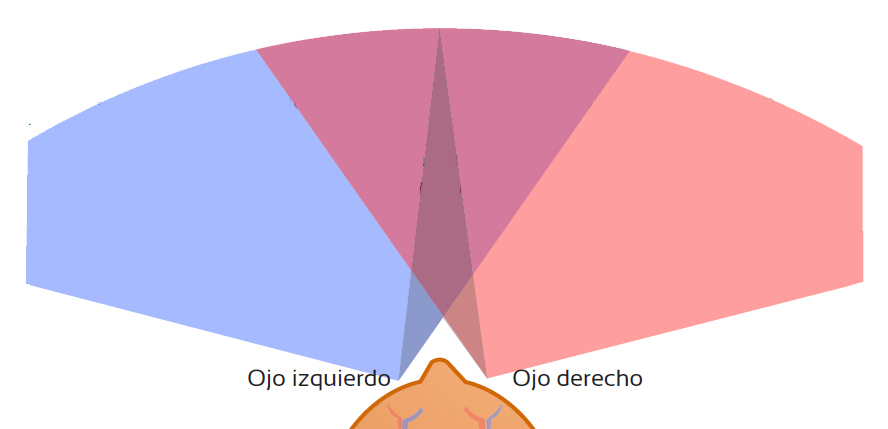
\includegraphics[scale=0.45]{Imagenes/Campo_visual_01.jpg}
     \caption{Superposición de los campos visuales de cada ojo.}
\end{figure}

Una vez que se tiene los campos visuales de ambos ojos, el alumno que mantenía el plumón, deberá de ser ahora el alumno que se cubrirá el ojo.
\par
Esta práctica realiza la técnica de campimetría cualitativa, es decir, el registro del campo visual es solo de manera general, no se debe de utilizar como una prueba clínica para determinar alguna situación o estado de salud visual.
\end{document}